% this is a comment in latex
% substitute this documentclass definition for uncommented one
% to switch between single and double column mode
\documentclass[11pt,twocolumn]{article}
%\documentclass[11pt]{article}

\usepackage{fullpage}
\usepackage{subfigure,indentfirst}
% for url
\usepackage{hyperref}
% for underlined text
\usepackage[normalem]{ulem}
% for including pdf figures
\usepackage{graphicx}
% tables
\usepackage[table,xcdraw]{xcolor}
\usepackage{clrscode3e}
% path to referenced images
\graphicspath{{images/}}

% my own versions: my_enumerate and my_itemize
\newenvironment{my_enumerate}{
  \begin{enumerate}
    \setlength{\itemsep}{1pt}
      \setlength{\parskip}{0pt}
\setlength{\parsep}{0pt}}{\end{enumerate}
}

\newenvironment{my_itemize}{
  \begin{itemize}
    \setlength{\itemsep}{1pt}
      \setlength{\parskip}{0pt}
\setlength{\parsep}{0pt}}{\end{itemize}
}

% this starts the document
\begin{document}

\title{Widening the Sieve: Parallelizing the Sieve of Eratosthenes}

\author{Richard Muniu, Michael Haregot, Kevin Zheng \\
Computer Science Department, Swarthmore College, Swarthmore, PA  19081}

\maketitle

\begin{abstract}
A prime number is a natural number greater than one that has no other factors 
rather than one and itself. Prime numbers have a variety of applications in 
multiple fields ranging from hashing and public-key cryptography, to mathematical 
research and quantum computing. Large primes, in particular, are crucial for 
security in cryptography, and the generation of such primes is a hot topic as 
a result. Since the distribution of prime numbers over a given interval is to 
this day still unknown, there exist a range of algorithms that allow us to 
generate 
these primes efficiently. In this paper, we focus on prime number sieves, 
specifically the Sieve of Eratosthenes, which provides a simple and relatively 
fast method of generating primes from zero up to a maximum positive integer 
$n$. Although this sieve is not embarrassingly parallel, we investigate 
different parallelization approaches using OpenMP, balanced pthreads, 
and CUDA across different interval sizes. We then compare the results from 
these implementations to determine their efficiency in terms of speedup. 
Our results demonstrate that although only part of our algorithm can be 
parallelized, there is a much to gain in efficiency from applying carefully 
constructed parallelism to generate these primes.

% The abstract is a brief summary of your work. It should be written to make the
% reader want to read the rest of your paper. Briefly state the basic contents
% and conclusions of your paper: the problem you are solving, why the reader
% should care about this problem, your unique solution and/or implementation,
% and the main results and and contributions of your work.

%   For writing organization resources, see my
%   CS Research and Writing Guide:

% \noindent {\small \url{www.cs.swarthmore.edu/~newhall/thesisguide} } 

% And, off my help pages~\cite{newhall:help} are links to other resources 
% for technical writing, including a writing style guide and information
% about Unix tools for creating and editing figures.  

\end{abstract}


\section {Introduction} 

% Introduction 


% The introduction is the big picture of your work: what, why, and how. It
% includes a definition of the problem you are solving, a high-level description
% of your solution including any novel techniques and results you provide, and a
% summary of the main results of your paper. In addition, motivates the problem
% you are solving (why should a reader find your work important), and describes
% your contribution to the area (this may not be applicable to your project).
% The first paragraph of the introduction should contain all of this information
% in a very high-level. Subsequent paragraphs should discuss in more detail the
% problem you are solving, your solution, and your results and conclusions.

Prime numbers have puzzled mathemeticians for centuries, and to this day there
remains no obvious method of quickly identifying them. The difficulty associated 
with finding large prime numbers has been exploited to create a variety of 
encryption techniques, making the discovery of large prime numbers essential 
for the safeguarding of private information. In this paper, we explore, implement, and
measure three different approaches to parallelizing a popular algorithm
for finding prime numbers.

Prime numbers have become so central to our lives primarily due
to two of their properties. For one, they are difficult to find. If handed
any arbitrary positive integer $N$, it can take significant work
to discover whether or not $N$ is a prime number. The aforementioned process is called
a \textit{primality test}, and there have been many such tests
that have been developed and proven, although they are beyond the
scope of this paper. For now, we shall just say that primality tests
are often slow to perform on very large numbers.

A second property that makes prime numbers so important is that it is very
easy to multiply them together, but very difficult to factor their product.
The second property and its one-way difficulty is what gives inspiration for
encryption algorithms that can easily encrypt messages, but are difficult to 
decrypt without knowing the correct key. One notable example is the Rivest-Shamir-Adleman
(RSA) algorithm, which uses ``two large secret prime numbers'' to create
encryption keys~\cite{RSA}.

While RSA encrytion has only been around relatively recently, people
have been searching for prime numbers for millenia. An algorithm
developed over 2000 years ago remains one of the most efficient
methods for finding prime numbers today. This algorithm, which is the focus
of our paper, is called the Sieve of Eratosthenes.

The idea behind the sieve is actually very simple. The input to the
algorithm is a positive integer $n$, and the output is a list
of all prime numbers less than $n$. To start, we allocate an array
of size $n$, where all values begin unmarked. We mark buckets $0$ and
$1$ as nonprime, then continue to iterate through the array starting at 
position
$2$. Whenever we encounter an array bucket at position $i$ that is
unmarked, we proceed to mark all array buckets that are multiples
of $i$. By the time the algorithm is complete, any unmarked number
is a prime number. The time complexity of the algorithm has been
shown to be $O(n\ln{\ln{n}})$~\cite{Wirian}.

The sequential algorithm is very effective, but it has the potential
to be made much faster by parallelization. In this paper, we explore
3 different methods of parallelization and measure the efficacy of
each one.


\section {Related Work}\label{relwork}
% This is an essential part of a research paper; discussing related work is a
% good way to put your work in context with other similar work, and to provide a
% way for you to compare/ contrast your work to other's work.  You should use
% feedback on the annotated bibliography from your project proposal to structure
% this section; it should be written as a re-write of your annotated bibliography
% in a single Related Work section.

There have been many previous attempts to parallelize the Sieve with
varying results. There was a paper by NASA in 1986 that shows that they
used the Sieve as a parallel benchmark test for their multicore
machines~\cite{Bohkari}.
They used a parallelization scheme in which they delegated a process to
marking all of the multiples of a prime; for example, they might have
one process marking all the multiples of 2 while another process marks
all the multiples of 3. They saw significant speedups, but only up until
about 4 or 5 processors. One problem that they specified was that their
approach was usually bound by the speed of the slowest process, since
processes marking off multiples of small primes had much more work
to do than processes marking off multiples of large primes.

We found a different approach detailed in 2014 paper called
\textit{Parallelization of Sieve of Eratosthenes}\cite{Bhat}.
Here, the authors
separated the array of numbers such that each process was responsible
for a contiguous block of the array. The first process would always
be responsible for first $\sqrt{n}$ numbers. The first process would
find a base prime number, then broadcast it to all of the other
processes. All processes would then proceed to mark all numbers
that are multiples of the broadcasted prime within their assigned
chunks. The use of broadcast avoids some of the load imbalance 
problems from the NASA
paper, but also introduces a few new ones, such as how each process
can efficiently determine which numbers in its chunk are multiples of
a number.


\section {Solution}\label{soln}
% Details of the problem you are solving Details of your solution and the
% project's implementation Even though you may have spent an enormous amount of
% time writing code, this should not include a listing of any code you wrote.
% Only if your project is about developing an algorithm or a new language, may
% code examples be appropriate here.  Discussion of how your solution solves the
% problem.

In order to compare and test different approaches, we implemented four
different versions of the Sieve of Eratosthenes. These are sequential
sieve, OpenMP sieve, balanced pthreads sieve, and CUDA sieve.

\subsection{Sequential Sieve}\label{seqsection}

Our first implementation was a sequential one. The program was written in C
and allowed the user to specify an input value $n$, such that the program
would find all prime numbers up to $n$. The pseudocode for the algorithm
is specified in Figure~\ref{seqpseud}. The sequential algorithm 
was useful since all of our other implementations use the algorithm
as a starting point, and we modified parts of the sequential code in order to
effectively parallelize it. The sequential implementation was also useful as
a benchmark when we began testing.

\begin{figure}
    \begin{codebox}
        \Procname{\proc{SequentialSieve}(n)}
        \li arr = array of size $n$
        \li \kw{for} element i in arr
        \Do
            \li i = PRIME
        \End
        \li arr[0] = NONPRIME
        \li arr[1] = NONPRIME
        \li \kw{for} i from $2$ to $\sqrt{n}$
        \Do
            \li \If arr[i] == NONPRIME
            \Do
                \li base = i
                \li next = base + base
                \li \kw{while} next $< n$
                \Do
                    \li arr[next] = NONPRIME
                    \li next = next + base
                \End
            \End
        \End
        \li return arr
    \end{codebox}
    \caption{{\label{seqpseud}} Pseudocode for our sequential implementation
    of the Sieve of Eratosthenes.}
\end{figure}

\subsection{OpenMP Sieve}\label{openmpsection}

Our OpenMP implementation was very similar to our sequential version. In fact,
we set these two versions to compile from the same source file, just with a
few extra lines of code for the OpenMP version. Instead of reproducing
the same pseudocode again, we can imagine that the OpenMP implementation's
pseudocode is the same as the sequential one's with the exception
that the \textit{for} loop on line 6 is instead a \textit{parallel for}.

OpenMP provides these parallel loops with very little intervention needed
from the programmer. The library essentially breaks up each iteration
of the loop into a different job, then assigns the jobs to an army
of processes that it forks off. In terms of our algorithm, the parallel for
loop means that each value of ``base'' is assigned to a thread, and that thread
proceeds to mark all multiples of its assigned ``base'' as nonprime.

Before we started writing our OpenMP implementation, we already expected
a few difficulties. By far the biggest one was that we suspected that
the implementation would suffer from imbalanced load problems. Similar,
to the issues described by Bohkari in his paper for NASA~\cite{Bohkari}.
As we discussed in section~\ref{relwork}, jobs with small bases
are much harder than jobs with large bases. The first iteration of
our implementation suffered heavily from imbalanced load. We soon found out that
the issue was being compounded by OpenMP's default static scheduling
method, which assigned the lowest iterations of the loop to one process,
the next lowest to the next process, and so on. Default static scheduling
resulted in the lowest number process being assigned all of the hardest
work in the batch. In order to fix the imbalance of work, we used OpenMP's 
dynamic scheduling instead, which causes jobs to be assigned as processes 
finish previous jobs. Dynamic scheduling provided some load balancing for us,
and massively improved the efficiency of our program.

It is worth noting that the OpenMP implementation has the potential
to do unnecessary and redundant work. For example, if a process
is assigned to the base value of $4$, it might identify it as
prime and start marking off its multiples before the process assigned
to the base of $2$ has the chance to mark $4$ as nonprime. Potential
overlap is just a cost that we have to live with, since having 
each process wait for all the other processes to reach a certain point 
would force the program to be so slow and so synchronized that it is
basically sequential.


\subsection{CUDA Sieve}\label{cudasection}

Our CUDA implementation was designed to be very similar to our OpenMP
implementation while taking advantage of the massive parallelism offered
by GPUs. The pseudocode is described in Figure~\ref{cudapseud}. Just as
OpenMP implicitly parallelized each iteration of a loop, here we
more explicitly parallelized each iteration of the same loop
using a CUDA kernel call. When the kernel is invokes,
\texttt{numthreads} threads are spawned and each begins executing the
code in the kernel. Each thread individually figures out which
value of \texttt{base} it is responsible for, then proceeds to mark
off all multiples of that base.

\begin{figure}
    \begin{codebox}
        \Procname{\proc{CUDASieve}(n)}
        \li arr = array of size $n$
        \li \kw{for} element i in arr
        \Do
            \li i = PRIME
        \End
        \li arr[0] = NONPRIME
        \li arr[1] = NONPRIME
        \li maxblock = max \# of thread blocks 
        \li maxthread = max \# of threads per block
        \li numthreads = maxblock * maxthread
        \li \kw{for} i from 0 to $\sqrt{n}/$numthreads
        \Do
            \li // call with maxblock blocks
            \li // and maxthread blocksize
            \li SieveKernel(arr, n, i*numthreads)
        \End
        \li return arr
    \end{codebox}
    \begin{codebox}
        \Procname{\proc{SieveKernel}(arr, n, start)}
        \li // this is CUDA kernel function
        \li base = start + blockID + threadID
        \li \If base == 0 or base == 1 
        \li or base $>\sqrt{n}$ or base == NONPRIME
        \Do
            \li return
        \End
        \li next = base + base
        \li \kw{while} next $< n$
        \Do
            \li arr[next] = NONPRIME
            \li next = next + base
        \End
        \li return
    \end{codebox}
    \caption{{\label{cudapseud}} Pseudocode for our CUDA implementation
    of the Sieve of Eratosthenes.}
\end{figure}

We have our kernel call in a loop in order to handle hardware limitations
on the number of threads that can be created at once. Each call to
the kernel creates as many threads as the GPU will allow, and once
they are finished, the next call does it again, this time assigning
the threads work that was not completed by the previous call.

When we first started testing, we expected the CUDA implementation
to perform the best. GPGPUs give access to a much higher degree
of parallelism than is otherwise possible on a CPU. While we may
be able to run 32 simultaneous processes on a machine with that
many CPUs, a GPU can often support hundreds of thousands or even millions
of simultaneous threads. We also felt that a GPU's Single Instruction
Multiple Data (SIMD) architecture would be perfect for tackling parallelization
of the Sieve of Eratosthenes. The SIMD architecture means that a GPU is 
most efficient when different threads are performing the same operation. 
As can be seen from the pseudocode in Figure~\ref{cudapseud}, there
is very little conditional branching in the kernel, meaning that our 
threads are almost always performing the same operations in the same order.

Similar to OpenMP, we expect our CUDA implementation to do significant
unnecessary and redundant work. For example, it is entirely possible
for the thread responsible for base $4$ to proceed with marking off
multiples since the thread responsible for base $2$ has the chance to
mark $4$ as nonprime. However, thanks to the GPU's SIMD architecture,
we do not anticipate that such potential overlap would slow down the 
program, since all the extra work is being executed in lockstep with 
all the necessary work at no extra cost.

\subsection{Balanced Pthreads Sieve}\label{balsection}

In an attempt to solve the problem of imbalanced workloads, we also created
a balanced pthreads solution. The balanced pthreads solution takes a 
fundamentally different approach at parallelizing the Sieve of Eratosthenes. 
Instead of having each thread separately handle a different base, 
we have a master thread that finds all of the bases, then broadcasts 
them to a group of worker threads. The master thread is assigned the 
first $\sqrt{n}$ elements of the array while the worker threads evenly divide 
the remaining pieces of the array between them. Every time the master 
broadcasts a base, each worker then identifies and marks all multiples of
the broadcasted base within its assigned section of the array. The
pseudocode is described in Figure~\ref{balpseud}.

\begin{figure}
    \begin{codebox}
        \Procname{\proc{BalSieve}(n, p)}
        \li arr = array of size $n$
        \li spawnThread(runMasterLoop(arr, n))
        \li \kw{for} i from 1 to $p-1$
        \Do
            \li spawnThread(runWorkerLoop(arr, n))
        \End
        \li joinAllThreads()
        \li return arr
    \end{codebox}
    \begin{codebox}
        \Procname{\proc{runMasterLoop}(arr, n)}
        \li initArrSection(0, $\sqrt{n}$)
        \li \kw{for} i from $2$ to $\sqrt{n}$
        \Do
            \li \If arr[i] == NONPRIME
            \Do
                \li base = i
                \li // inform other threads
                \li broadcast(base)
                \li next = base + base
                \li \kw{while} next $< \sqrt{n}$
                \Do
                    \li arr[next] = NONPRIME
                    \li next = next + base
                \End
            \End
        \End
        \li broadcast(done)
    \end{codebox}
    \begin{codebox}
        \Procname{\proc{runWorkerLoop}(arr, n)}
        \li start, end = getBounds()
        \li initArrSection(start, end);
        \li \kw{while} true
        \Do
            \li // get value from master
            \li base = recvBroadcast()
            \li \If base == done
            \Do
                \li return
            \End
            \li next = firstMultiple(start, end, base)
            \li \kw{while} next $< n$
            \Do
                \li arr[next] = NONPRIME
                \li next = next + base
            \End
        \End
    \end{codebox}
    \caption{{\label{balpseud}} Pseudocode for our balanced
    pthreads implementation of the Sieve of Eratosthenes.}
\end{figure}

The pseudocode is less explicit than in our previously mentioned
pseudocode because there are a lot of implementation details
here that would take too long to fully detail. There are still
some details here that are worth going over though.

The input value $p$ is the number of threads the user wants to spawn,
including the master thread. When $p = 1$, the balanced pthreads 
algorithm is functionally equivalent to sequential sieve.

In \texttt{getBounds}, the runtime of this function is $O(p)$, and it
equally splits the data between the worker threads such that each
worker is responsible for a contiguous chunk of the array.

In \texttt{recvBroadcast}, the information is propagated using a shared
memory variable and and synchronized using a barrier. The synchronization 
introduces some waiting overhead to the algorithm and forces the master 
and workers to all be done working on one base before they can move 
on to the next base.

In \texttt{firstMultiple}, modulus math is used to find the first
multiple of the base within the section of the array in $O(1)$ time.

The main advantage of the balanced pthreads approach is how it 
evenly distributes work among the threads. The only potential source of 
imbalance is the portion of the array that the master thread is responsible. 
After the master finds a base, it essentially acts like a worker thread 
and fills in all of the multiples for its own portion of the array. 
However, since the master is always responsible for approximately 
$\sqrt{n}$ elements, it may have more or less filling it to do than 
the worker threads. Optimally, $n$ and $p$ should be balanced so that the
master's portion of the array is not too drastically different from 
the other threads' portions.

One nice property of balanced pthreads is that unlike our OpenMP and CUDA
implementations, it never wastes work. Since the master is responsible for
sequentially finding all bases, it knows when a base has or has not
already been marked off.

\subsection{Other Approaches}\label{othersection}

There are many different ways to parallelize the Sieve of Eratosthenes
that we did not try. Most notably, all of our solutions confine the program
to a single running machine with no attempt to communicate between
multiple machines. We recognize that this means we have sacrificed the
ability to take full advantage of large clusters, but we believe there
is good reason to stay on one machine. The key insight here is that
the calculation in the Sieve algorithm is fundamentally very simple, so any
additional overhead incurred can be a significant portion of runtime. At
its heart, the calculation being performed here is repeated addition,
multiplication, and writes to memory. An implementation that ran across
a cluster of machines would suffer heavily from the cost of communicating
across a network. Additionally, results would need to be aggregated
at the end of the run, and if a master node had to read over the results
from each individual machine and write them to a final copy, all of these
reads and writes may actually end up being a very large part of the runtime.

To show just how costly communication would be, imagine master node 
that has tasked another node to mark off all multiples of some base $x$. 
In order to complete this task, the worker node would have to complete approximately
$n/x$ multiplication and $n/x$ writes to its local memory. On a shared
memory system, that would be the end of the story, but in a distributed
system, these results need to be sent over the network back to the master.
We can abstract the communication as $n/x$ writes to the network and $n/x$ reads
from the network. The master then has to write the new results into
its own memory, resulting in another $n/x$ writes to memory. Since
memory access and network usage is relatively expensive compared to
multiplication, it can be seen that distributing the Sieve of Eratosthenes
across multiple machines can be very expensive.

That is not to say it is not possible to distribute the sieve and take
advantage of a cluster, but in this paper we simply chose to pursue the
techniques that we thought most promising, which is why we chose to
only use systems with shared memory.

\section {Results}\label{results}
% Experimental Results demonstrating/proving your solution Explain the tests you
% performed (and why) Explain how you gathered the data and details of how your
% experiments were run (any system/environment set up) Present your results
% Choose quality over quantity; the reader will not be impressed with pages and
% pages of graphs and tables, instead s/he wants to be convinced that your
% results show something interesting and that your experiments support your
% conclusions.  Discuss your results!  Explain/interpret your results (possibly
% compare your results to related work). Do not just present data and leave it up
% to the reader to infer what the data show and why they are interesting.  
For this project, we chose to assess how our implementations scale
in relation to the task size rather than the number
of processors. Scaling the workload rather than the number of processors
made it easier to compare implementations across
architectures that do not have much in common, as is the case for CPU and GPGPU
computing. The following subsections detail our test methods and their related
results, which we discuss in a later subsection.

\subsection{OpenMP}
We ran three rounds of tests for our OpenMP implementation on the high-memory
(\texttt{himem-01}) partition of Swarthmore's Strelka cluster, and collected 
and aggregated these values. Tables~\ref{seq1runtime} and~\ref{openmpruntime} 
show the output for sequential and parallel runs of the Sieve algorithm
respectively, for array sizes ranging from size $10$ to $10^{12}$. Our runs were kept to
arrays of size $10^{12}$ due to RAM limitations that caused \texttt{malloc} errors
for array sizes of $10^{13}$ and above.

\begin{table}[]
\centering
\begin{tabular}{|l|l|l|}
\hline
\begin{tabular}[c]{@{}l@{}}Size\\ (10\textasciicircum{}\{x\})\end{tabular} & \begin{tabular}[c]{@{}l@{}}Average\\ Sequential\\ Runtime\end{tabular} & Variance \\
\hline
1 & 0.005 & 0.000 \\
2 & 0.001 & 0.000 \\
3 & 0.001 & 0.000 \\
4 & 0.001 & 0.000 \\
5 & 0.001 & 0.000 \\
6 & 0.007 & 0.000 \\
7 & 0.071 & 0.000 \\
8 & 2.204 & 0.102 \\
9 & 27.518 & 0.124 \\
10 & 308.638 & 20.314 \\
11 & 3364.497 & 448.690 \\
\hline
\end{tabular}
\caption{Sequential Sieve Runtime in Seconds}
\label{seq1runtime}
\end{table}

\begin{table}[]
\centering
\begin{tabular}{|l|l|l|}
\hline
\begin{tabular}[c]{@{}l@{}}Size\\ (10\textasciicircum{}\{x\})\end{tabular} & \begin{tabular}[c]{@{}l@{}}Average\\ Parallel\\ Runtime\end{tabular} & Variance \\
\hline
1 & 0.017 & 0.000 \\
2 & 0.016 & 0.000 \\
3 & 0.017 & 0.000 \\
4 & 0.016 & 0.000 \\
5 & 0.018 & 0.000 \\
6 & 0.017 & 0.000 \\
7 & 0.027 & 0.000 \\
8 & 0.201 & 0.000 \\
9 & 1.923 & 0.001 \\
10 & 19.372 & 0.237 \\
11 & 216.177 & 100.482 \\
\hline
\end{tabular}
\caption{OpenMP Sieve Runtime in Seconds}
\label{openmpruntime}
\end{table}

Using these values, we computed the related speedup for each of the
array sizes, shown in Table~\ref{openmpspeedup}, to assess the 
relative performance of our our two algorithms in processing the 
same task at different scales. Our 
OpenMP implementation achieved speedups of up to 16. 

\begin{table}[]
\centering
\begin{tabular}{|l||l|l||l|}
\hline
\begin{tabular}[c]{@{}l@{}}Size \\ ($10^x$)\end{tabular} & \begin{tabular}[c]{@{}l@{}}Average\\ Sequential\\ Time(s)\end{tabular} & \begin{tabular}[c]{@{}l@{}}Average\\ Parallel\\ Time(s)\end{tabular} & Speedup\\
\hline
1                                                       & 0.001                                                        & 0.017                                                        & \cellcolor[HTML]{F4CCCC}{\color[HTML]{000000} 0.058}  \\
2                                                       & 0.001                                                        & 0.016                                                        & \cellcolor[HTML]{F4CCCC}{\color[HTML]{000000} 0.063}  \\
3                                                       & 0.001                                                        & 0.017                                                        & \cellcolor[HTML]{F4CCCC}{\color[HTML]{000000} 0.059}  \\
4                                                       & 0.001                                                        & 0.016                                                        & \cellcolor[HTML]{F4CCCC}{\color[HTML]{000000} 0.061}  \\
5                                                       & 0.001                                                        & 0.018                                                        & \cellcolor[HTML]{F4CCCC}{\color[HTML]{000000} 0.057}  \\
6                                                       & 0.008                                                        & 0.017                                                        & \cellcolor[HTML]{F4CCCC}{\color[HTML]{000000} 0.462}  \\
7                                                       & 0.073                                                        & 0.027                                                        & \cellcolor[HTML]{B6D7A8}{\color[HTML]{000000} 2.750}  \\
8                                                       & 2.050                                                        & 0.201                                                        & \cellcolor[HTML]{B6D7A8}{\color[HTML]{000000} 10.182} \\
9                                                       & 27.495                                                       & 1.923                                                        & \cellcolor[HTML]{B6D7A8}{\color[HTML]{000000} 14.298} \\
10                                                      & 308.771                                                      & 19.372                                                       & \cellcolor[HTML]{B6D7A8}{\color[HTML]{000000} 15.939} \\
11                                                      & 3371.608                                                     & 216.177                                                      & \cellcolor[HTML]{B6D7A8}{\color[HTML]{000000} 15.596} \\
\hline
\end{tabular}
\caption{OpenMP vs Sequential Sieve speedup}
\label{openmpspeedup}
\end{table}

\subsection{Balanced Pthreads}
As with the OpenMP parallelization tests, we ran three rounds of tests
for our balanced pthreads implementation on the high-memory partition
of Swarthmore's Strelka cluster, and collected and aggregated the values.
Tables~\ref{seq2runtime} and~\ref{balruntime} below show the output for
sequential and parallel runs of the Sieve algorithm respectively, for array
sizes ranging from size $10$ to $10^{12}$. The array sizes were also capped
at $10^{12}$ as in the OpenMP case due to RAM limitations that prevented
dynamic allocation of arrays of size $10^{13}$ and above.

\begin{table}[]
\centering
\begin{tabular}{|l|l|l|}
\hline
\begin{tabular}[c]{@{}l@{}}Size\\ (10\textasciicircum{}\{x\})\end{tabular} & \begin{tabular}[c]{@{}l@{}}Average\\ Sequential\\ Runtime\end{tabular} & Variance \\
\hline
1 & 0.005 & 0.000 \\
2 & 0.001 & 0.000 \\
3 & 0.001 & 0.000 \\
4 & 0.001 & 0.000 \\
5 & 0.001 & 0.000 \\
6 & 0.007 & 0.000 \\
7 & 0.071 & 0.000 \\
8 & 2.204 & 0.102 \\
9 & 27.518 & 0.124 \\
10 & 308.638 & 20.314 \\
11 & 3364.497 & 448.690 \\
\hline
\end{tabular}
\caption{Sequential Sieve Runtime in Seconds}
\label{seq2runtime}
\end{table}

\begin{table}[]
\centering
\begin{tabular}{|l|l|l|}
\hline
\begin{tabular}[c]{@{}l@{}}Size\\ (10\textasciicircum{}\{x\})\end{tabular} & \begin{tabular}[c]{@{}l@{}}Average\\ Parallel\\ Runtime\end{tabular} & Variance \\
\hline
1 & 0.002 & 0.000 \\
2 & 0.002 & 0.000 \\
3 & 0.003 & 0.000 \\
4 & 0.005 & 0.000 \\
5 & 0.009 & 0.000 \\
6 & 0.016 & 0.000 \\
7 & 0.046 & 0.000 \\
8 & 0.228 & 0.002 \\
9 & 2.440 & 0.014 \\
10 & 18.786 & 0.934 \\
11 & 199.944 & 28.580 \\
\hline
\end{tabular}
\caption{Balanced pthread Sieve Runtime in Seconds}
\label{balruntime}
\end{table}

The associated speedup for different array sizes is shown in Table~\ref{balspeedup}. Our balanced pthread implementation had quite similar performance to the OpenMP implementation, and had a maximum speedup of about 16.

\begin{table}[]
\centering
\begin{tabular}{|l||l|l||l|}
\hline
\begin{tabular}[c]{@{}l@{}}Size \\ ($10^x$)\end{tabular} & \begin{tabular}[c]{@{}l@{}}Average\\ Sequential\\ Runtime\end{tabular} & \begin{tabular}[c]{@{}l@{}}Average\\ Parallel\\ Runtime\end{tabular} & Speedup\\
\hline
1                                                       & 0.005                                                        & 0.002                                                        & \cellcolor[HTML]{B6D7A8}{\color[HTML]{000000} 2.500}  \\
2                                                       & 0.001                                                        & 0.002                                                        & \cellcolor[HTML]{F4CCCC}{\color[HTML]{000000} 0.429}  \\
3                                                       & 0.001                                                        & 0.003                                                        & \cellcolor[HTML]{F4CCCC}{\color[HTML]{000000} 0.375}  \\
4                                                       & 0.001                                                        & 0.005                                                        & \cellcolor[HTML]{F4CCCC}{\color[HTML]{000000} 0.200}  \\
5                                                       & 0.001                                                        & 0.009                                                        & \cellcolor[HTML]{F4CCCC}{\color[HTML]{000000} 0.154}  \\
6                                                       & 0.007                                                        & 0.016                                                        & \cellcolor[HTML]{F4CCCC}{\color[HTML]{000000} 0.458}  \\
7                                                       & 0.071                                                        & 0.046                                                        & \cellcolor[HTML]{B6D7A8}{\color[HTML]{000000} 1.547}  \\
8                                                       & 2.204                                                        & 0.228                                                        & \cellcolor[HTML]{B6D7A8}{\color[HTML]{000000} 9.653}  \\
9                                                       & 27.518                                                       & 2.440                                                        & \cellcolor[HTML]{B6D7A8}{\color[HTML]{000000} 11.278} \\
10                                                      & 308.638                                                      & 18.786                                                       & \cellcolor[HTML]{B6D7A8}{\color[HTML]{000000} 16.429} \\
11                                                      & 3364.497                                                     & 199.944                                                      & \cellcolor[HTML]{B6D7A8}{\color[HTML]{000000} 16.827} \\
\hline
\end{tabular}
\caption{Balanced pthread speedup}
\label{balspeedup}
\end{table}

\subsection{CUDA}
Finally, as with out two other parallel implementation tests,
we ran three rounds of tests for our CUDA implementation on the GPU partition
(\texttt{gpu-02}) of Swarthmore
College's Strelka cluster, and collected and aggregated the values. Table 7
below shows the output for only parallel runs of the Sieve algorithm for
array sizes ranging from size $10$ to $10^{12}$. Since our previous
sequential runs showed stable performance with a low standard deviation, 
in this case we chose to use the average of our pre-calculated average
runtimes for the sequential sieve implementation  to compare against our 
CUDA implementation runtime. While our array sizes were capped at 
$10^{12}$ in our previous implementations (sequential, OpenMP, and balanced
pthreads), we were limited here by GPU memory, where \texttt{cudaMalloc} 
failed for arrays of size greater than or equal to $10^{11}$. 
Table~\ref{cudaruntime} shows the runtime of our CUDA sieve for array sizes
from $10^1$ to $10^{11}$.

\begin{table}[]
\centering
\begin{tabular}{|l|l|l|}
\hline
\begin{tabular}[c]{@{}l@{}}Size\\ (10\textasciicircum{}\{x\})\end{tabular} & \begin{tabular}[c]{@{}l@{}}Average\\ Parallel\\ Runtime\end{tabular} & Variance \\
\hline
1 & 3.128 & 0.005 \\
2 & 3.039 & 0.000 \\
3 & 3.060 & 0.000 \\
4 & 3.057 & 0.002 \\
5 & 3.076 & 0.000 \\
6 & 3.090 & 0.003 \\
7 & 3.295 & 0.007 \\
8 & 4.536 & 0.000 \\
9 & 17.802 & 0.002 \\
10 & 158.962 & 0.084 \\
11 & - & - \\
\hline
\end{tabular}
\caption{CUDA Sieve Runtime in Seconds}
\label{cudaruntime}
\end{table}

The speedup for our CUDA implementation over different array sizes 
is shown in Table~\ref{cudaspeedup}. We shall discuss these results
in the next section.

\begin{table}[]
\begin{tabular}{|l||l|l||l|}
\hline
\begin{tabular}[c]{@{}l@{}}Size \\ ($10^x$)\end{tabular} & \begin{tabular}[c]{@{}l@{}}AVERAGE\\ SEQ\\ TIME\end{tabular} & \begin{tabular}[c]{@{}l@{}}AVERAGE\\ PAR\\ TIME\end{tabular} & Speedup \\
\hline
{\color[HTML]{000000} 1} & 0.005 & 3.128 & \cellcolor[HTML]{F4CCCC}{\color[HTML]{000000} 0.002} \\
{\color[HTML]{000000} 2} & 0.001 & 3.039 & \cellcolor[HTML]{F4CCCC}{\color[HTML]{000000} 0.000} \\
{\color[HTML]{000000} 3} & 0.001 & 3.060 & \cellcolor[HTML]{F4CCCC}{\color[HTML]{000000} 0.000} \\
{\color[HTML]{000000} 4} & 0.001 & 3.057 & \cellcolor[HTML]{F4CCCC}{\color[HTML]{000000} 0.000} \\
{\color[HTML]{000000} 5} & 0.001 & 3.076 & \cellcolor[HTML]{F4CCCC}{\color[HTML]{000000} 0.000} \\
{\color[HTML]{000000} 6} & 0.007 & 3.090 & \cellcolor[HTML]{F4CCCC}{\color[HTML]{000000} 0.002} \\
{\color[HTML]{000000} 7} & 0.071 & 3.295 & \cellcolor[HTML]{F4CCCC}{\color[HTML]{000000} 0.021} \\
{\color[HTML]{000000} 8} & 2.204 & 4.536 & \cellcolor[HTML]{F4CCCC}{\color[HTML]{000000} 0.486} \\
{\color[HTML]{000000} 9} & 27.518 & 17.802 & \cellcolor[HTML]{B6D7A8}{\color[HTML]{000000} 1.546} \\
{\color[HTML]{000000} 10} & 308.638 & 158.962 & \cellcolor[HTML]{B6D7A8}{\color[HTML]{000000} 1.942} \\
{\color[HTML]{000000} 11} & - & - & - \\
\hline
\end{tabular}
\caption{CUDA vs Sequential Sieve Speedup}
\label{cudaspeedup}
\end{table}

\subsection{Discussion}
We compared the runtimes of each of our three implementations against
each other in order to analyse the efficiency of each of our three parallel
algorithms. Figure~\ref{runtimecomp} shows a comparison of the sequential 
runtimes and parallel runtimes of our OpenMP, balanced pthreads, and CUDA 
implementations for different array sizes. 

\begin{figure*}
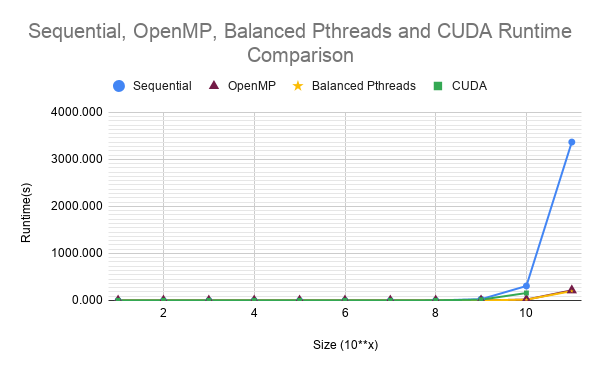
\includegraphics[width=15cm]{runtime-comp.png}
\caption{OpenMP, Balanced pthread, CUDA, and Sequential Sieve Runtime Comparison}
\label{runtimecomp}
\end{figure*}

Note that the balanced pthread and OpenMP runtimes are strikingly 
similar, and show up overlayed in the graph. The similarity is 
because OpenMP's dynamic scheduling construct assigns each iteration
of our prime number identification loop to a chunk, then lets each 
available thread execute
the iteration and request for more chunks until no chunks are left.
Effectively, dynamic scheduling balances the load among processors,
since no single thread gets assigned most of the heavy work such as
identification and striking off of small prime numbers like $2$,
$3$, and $5$. Dynamic scheduling effectively keeps all threads
engaged as much as possible while there remains work to be done.
In our balanced pthreads implementation, on the other hand, our master
thread is tasked with the job of finding the next available prime
number, and each slave thread is responsible for striking off nonprimes
in the section of the array for which it is responsible. This effectively 
spreads the work across all threads and ensures that all threads are 
as fully engaged as possible throughout the execution. 

Our CUDA implementation displayed the least performance improvement for
most array sizes, but demonstrated a slight improvement for arrays of
sizes $10^9$ and $10^{10}$. It's runtime remained slower than that of 
our sequential implementation, despite the availability of a large
number or blocks and threads per block. Because our kernel code does 
not seem complex, we hypothesize that that with the large sizes of
shared memory required to hold such large arrays, our application 
could be running into bank conflicts when consecutive threads in a
warp try to access consecutive or nearby addresses in shared memory.
A result of these conflicts would be serialized access to memory in
the cases where multiple addresses of a memory request map to a single 
bank. Additionally, the overhead from kernel invocation and copying
of data from the device to the host and vice versa could explain the 
high and relatively stable runtimes for small-sized arrays.  
Figure~\ref{speedupcomp} shows a comparision of the speedup from using
the different paralellization techniques (OpenMP, balanced pthreads,
and CUDA) across different array sizes. We used the figure to 
extrapolate and predict, based on our current performance, how much
these three implementations would benefit from parallelizaion in the
absence of memory bottlenecks. While it is difficult to see what 
happens beyond the $10^{11}-10^{12}$ range, it seems highly likely 
that our balanced pthread and OpenMP implementations would plateau 
around their maximum speed-up level.

\begin{figure*}
\centering
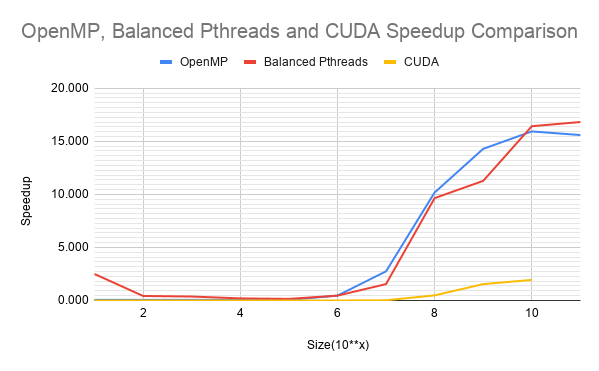
\includegraphics[width=15cm]{speedup-comp.png}
\caption{OpenMP, Balanced pthread, and CUDA Speedup Comparison}
\label{speedupcomp}
\end{figure*}

\section{Conclusions and Future Directions}\label{conc} 
% Conclusions and Future Directions for your work Conclude with the main ideas
% and results of your work. Discuss ways in which your project could be
% extended...what's next? what are the interesting problems and questions that
% resulted from your work?
While over 2000 years old, the Sieve of Eratosthenes has shown itself to be
a solid algorithm for generating prime numbers. In the modern age where multi-core 
processors are the norm, we have shown that a parallel approach offers large
improvements
in terms of speed and efficiency. In this paper, we implemented and evaluated
different
methods of parallelization using OpenMP, balanced pthreads, and CUDA.
Our results show solid improvements in performance, with speedups of up to
16. We did notice that while OpenMP and balanced pthreads sieves performed 
similarly well, our CUDA sieve did not offer as much speedup as the other two
implementations. This was contrary
to our initial expectations, as we thought that CUDA would be the
ideal tool for writing this algorithm. CUDA under-performed despite having
access to a massive number parallel threads. We are unsure if this is due
to hardware limitations, or rather due to
software optimizations that could have been included in our code.

There is still more work to be done in making these algorithms practical. For example, 
all of our approaches use simple linear sieving and use
$O(n)$ memory. As a result, we are limited by the maximum
memory capacity of a machine. Additionally, as the array sizes grow, 
memory access speed quickly becomes the computational bottleneck since we reap
less and less of the benefits of cache locality. Further work is needed to
develop, implement, and test versions of this algorithm that are more flexible
with their memory usage. Ideally, an algorithm would be able to de-allocate portions
of the array if it no longer needs them and write them to disk instead.

\section{Meta-discussion}\label{meta} 
% A brief meta-discussion of your project Include two paragraphs in this section:
% Discussion of what you found to be the most difficult and least difficult parts
% of your project.  In what ways did your implementation vary from your proposal
% and why?  

The most difficult of our work was the implementation of CUDA
while the least difficult was OpenMP. As mentioned previously,
OpenMP implementation was extremely similar to our sequential version and 
required little additional coding on our part outside of the using of
parallel loop primitives and a changing of scheduling from static from dynamic
to manage imbalance. Our CUDA implementation had memory issues where it
would run out of memory for arrays of size greater than $10^{11}$. Our results 
for the CUDA 
implementation were actually worse than our sequential version with the 
exception of arrays of $10^9$ and $10^{10}$ which made us question whether
there were issues with our code, or if that was the best performance CUDA 
could offer. 

We originally proposed to write only a CUDA implementation of the Sieve of 
Eratosthenes, however, we eventually branched off to include an OpenMP
and balanced pthreads implementation as well. This is because we realized
that it would be relatively easy to create an OpenMP implementation, and
that it would provide interesting insights to be able to compare
different approaches to each other. We created the balanced pthreads
implementation because we had read about a balanced data-parallel
approach in a paper and it seemed like a promising approach~\cite{Bhat}.


% At the end of your paper is a Reference section. You must cite each paper that
% you have referenced...your work is related to some prior work.

% The References section is auto generated by specifying the .bib file
% containing bibtex entries, and the style I want to use (plain)
% compiling with latex, bibtex, latex, latex, will populate this
% section with all references from the .bib file that I cite in this paper
% and will set the citations in the prose to the numbered entry here
\bibliography{finalreport}
\bibliographystyle{plain}

% force a page break
% \newpage 
% I want the Appendices to be single column pages
% \onecolumn
% \section{Appendices}\label{appx} 

% You may optionally add appendices to your report.  They do not count towards
% page total.  Appendicies are for expanding on details or results that are
% beyond inclusion in the main part of paper.  It could be where you have code
% snippets that illustrate some of details of what you discuss, but it is not a
% venue for a dump of all the code you wrote, which has no place in research
% paper.  


% \newpage
% \twocolumn
% \section{some latex examples}

% In my latex examples:
% \begin{verbatim}
% /home/newhall/public/latex_examples/paper/
% \end{verbatim}
% Is an example report and bibtex for a paper with lots of examples
% of latex formatting for tables, figures, references. etc.  See 
% the {\tt paper.tex} file and the {\tt paper.bib } file for lots of
% examples. Also, off my   help pages is some information for how to 
% convert documents from one form to another: 
% {\small \url{www.swarthmore.ed/~newhall/unixlinks.html#doc} }

% Here are a few latex examples:

% \subsubsection{Examples of figure and section references}

% To refer to a figure or section with a label, 
% use {\tt backslash ref\{labelname\}} and note where the labelname is 
% defined in the figure.  For example: (see Figure~\ref{dyncompex}, see 
% Section~\ref{meta}). 

% \subsubsection{Examples of incorporating figures}

% Here is an example of how to incorporate a figure in a document...you need
% to include a graphics package at the top of the latex document.  

% \begin{figure}[t]
% \centerline{\includegraphics[height=1.0in]{/home/newhall/public/latex_examples/report/ERbook.pdf}}

% \caption{ {\label{dyncompex} {\tt Figures should have a caption that 
%     describes what the figure is/shows}.  For example: During a dynamically 
%     compiled execution, methods may be interpreted by the VM and/or 
%     compiled into native code and directly executed. 
%     {\em The native code may still interact with the VM.  In this 
%       case, the VM acts like a run-time library to the AP.
% }}}
% \end{figure}

% {\bf For all figures in the document, you should refer to it and 
% describe what it shows in the prose of your paper}.  Here is an example: 
% Figure~\ref{dyncompex} shows the two execution modes of an 
% environment that uses dynamic compilation: (1) the VM interprets AP 
% byte-codes; (2) native code versions of AP methods, that the VM compiles 
% at run-time, are directly executed by the operating system/architecture 
% platform with some residual VM interaction (for example, activities like 
% object creation, thread 
% synchronization, exception handling, garbage collection, and calls from native 
% code to byte-code methods may require VM interaction). 

% \subsubsection {Figure Formating}

% I can force a figure to the top or bottom of a page by using the [t] or [b].
% I can also try to force it to come after the prose it follows in the .tex
% file by using [!htb] (latex doesn't always comply):

% \subsection {column spanning figures or tables}

% In two-column documents, you often have figures or tables that are
% too large to fit in a single column.  In this case you can specify
% that they fill both columns of the document by defining a table or 
% column with a {\tt *} at the end: {\tt figure*} or {\tt table*}. Latex
% will only place these at the very top or very bottom of a two-column
% document.   See Table~\ref{swapdevresults} for one example.  You can
% uncomment the following figure definition to generate another example:

% \begin{table*}
% \begin{center}
% \begin{tabular}{|l||r l|r|r|r|}
% \hline
% \multicolumn{1}{|c||}{Benchmark} & \multicolumn{2}{c|}{Nswap2L} &\multicolumn{1}{c|}{Nswap} &\multicolumn{1}{c|}{Flash} & \multicolumn{1}{c|}{Disk} \\
% \hline
% WL1   & {\bf 443.0} & (3.5 speedup)    & 471.8  & 574.2  & 1547.4 \\
% WL2   & {\bf 591.6} &(30.0)            & 609.7  & 883.1  & 17754.8\\
% WL4   & {\bf 578.9} &(30.9)            & 591.7  & 978.4  & 17881.2\\
% Radix & {\bf 110.7} &(2.3)             & 113.7  & 147.4  & 255.5 \\
% HPL   & 536.1 &(1.5)             & {\bf 529.7}  & 598.7  & 815.3 \\
% \hline
% \end{tabular}

% \caption{\label{swapdevresults} Comparison of different swap devices. 
%   {\em For each benchmark, the total run time (in seconds) when 
%     run using Nswap2L, Nswap Network RAM, flash or Disk as the 
%     swap partition. Bold entries show the best time.  Nswap2L speedups 
% over disk are in parentheses.} }
% \end{center}
% \end{table*}

% The first part of a tabular definition {\tt e.g. |c|l|r|rr|} 
% specifies the number of columns, the text alignment in each column,
% (centered, left, right), and any vertical bars you want drawn between 
% columns.  In this example, there are 3 columns, the first is 
% centered, the others right-aligned, and there is a double 
% vertical bar between the first and second columns and a single bar 
% between the second and third.

% Each row of values is listed on a separate line with.  Ampersands are 
% used between each column's value, and backslash-backslash ends a row.   
% {\tt hline} can be used to draw horizontal lines.  

% The second table definition is a larger example that 
% demonstrates the multicolumn directive
% which can be used to change the default formating of a particular row,
% including allowing content to span multiple columns, to be aligned 
% differently, and to have different vertical bars drawn then the 
% default column definitions listed in the tabular definition:



\end{document}
